\beginsong{Bella ciao}[wuw={nach einem italienischen Partisanenlied 1942, Übersetzung: Diether Dehm}, bo={33}, pfii={102}, index={An ihrer Schulter}]

\markboth{\songtitle}{\songtitle}

\beginverse
\endverse

\centering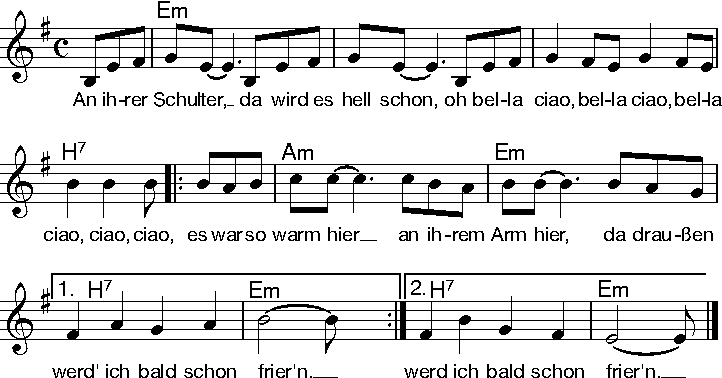
\includegraphics[width=1\textwidth]{Noten/Lied010.pdf}	

\beginverse
Kann nicht gut \[Em]schießen und krieg' schnell Angst auch,
o bella ciao, bella ciao, bella \[H7]ciao, ciao, ciao.
\lrep Soll ich ein \[Am]Held sein, dem das ge\[Em]fällt? Nein!
Verfluchter \[H7]Krieg, verfluchter \[Em]Feind! \rrep
\endverse
 
\beginverse
Sah Blut an ^Hütten, sah Frauen bitten,
o bella ciao, bella ciao, bella ^ciao, ciao, ciao.
\lrep Den kleinen ^Luca, der 14 ^Jahr' war,
ich hab zu ^lang nur zuge^seh'n. \rrep
\endverse

\beginverse
Ihr in den ^Bergen, heut' komm ich zu euch,
o bella ciao, bella ciao, bella ^ciao, ciao, ciao.
\lrep Was kein Kom^mando und kein Be^fehl kann:
Ich werde ^heute Parti^san. \rrep
\endverse

\beginverse
Wenn ich am ^Dorfplatz mal tot herumlieg',
o bella ciao, bella ciao, bella ^ciao, ciao, ciao,
\lrep dann sagt der ^Priester statt langer ^Predigt:
'Nie mehr Fa^schismus, nie mehr ^Krieg!' \rrep
\endverse

\beginverse
Nur noch der ^Kuss hier, kommt einer nach mir,
o bella ciao, bella ciao, bella ^ciao, ciao, ciao.
\lrep Dem wünsch' ich ^Zeiten, wo man so ^eine
wie dich nicht ^mehr verlassen ^muss. \rrep
\endverse

\endsong

\beginscripture{}
Diese Version des antifaschistischen Arbeiterliedes glorifiziert im Gegensatz zur anderen nicht den "Heldentod" der Partisanen.
\endscripture

\begin{intersong}

\end{intersong}